\documentclass[utf8]{ctexart}

\usepackage[a4paper,left=1.25in,right=1.25in,top=1in,bottom=1in]{geometry}
\usepackage{listings}
\usepackage{graphicx}
\usepackage{caption}
\usepackage{subfigure}
\usepackage{booktabs}
\usepackage{amsmath}
\usepackage{amsthm}
\usepackage{amsfonts}
\usepackage{float}
\usepackage{indentfirst}
\usepackage{tikz}
\usetikzlibrary{shapes,arrows}
\usetikzlibrary{shapes.geometric, arrows}
\usepackage{algorithm}
\usepackage{algorithmic}
\usepackage{newclude}
\usepackage[perpage]{footmisc}

\graphicspath{ {images/} }
\raggedbottom	% 令页面在垂直方向向顶部对齐
\renewcommand\qedsymbol{QED}
\newcommand{\sign}[1]{\mathrm{sgn}(#1)}
\everymath{\displaystyle}   % 行内公式采用行间公式格式排列
\pagestyle{plain}

\title{《计算机辅助几何设计》第五次作业}
\author{姓名:殷文良\qquad 学号:12435063}
\date{\today}

\begin{document}
\maketitle
\ctexset { section = { format={\Large \bfseries } } }

\section*{思考题 1}
\subsection*{1.}
\begin{proof}
    由$k$阶非均匀B样条基函数的定义,
    \begin{equation*}
        \begin{aligned}
            N_{i,3}(t) &= (t_{i+3}-t_i)\cdot [t_i,\cdots,t_{i+3}](\cdot-t)_+^2\\
            &= [t_{i+1},t_{i+2},t_{i+3}](\cdot-t)_+^2 - [t_{i},t_{i+1},t_{i+2}](\cdot-t)_+^2\\
            &= \frac{[t_{i+2},t_{i+3}](\cdot-t)_+^2 - [t_{i+1},t_{i+2}](\cdot-t)_+^2}{t_{i+3} - t_{i+1}} - \frac{[t_{i+1},t_{i+2}](\cdot-t)_+^2 - [t_{i},t_{i+1}](\cdot-t)_+^2}{t_{i+2} - t_{i}}\\
            &= \frac{\frac{(t_{i+3}-t)_+^2 - (t_{i+2}-t)_+^2}{t_{i+3}-t_{i+2}} - \frac{(t_{i+2}-t)_+^2 - (t_{i+1}-t)_+^2}{t_{i+2}-t_{i+1}}}{t_{i+3} - t_{i+1}}
            - \frac{\frac{(t_{i+2}-t)_+^2 - (t_{i+1}-t)_+^2}{t_{i+2}-t_{i+1}} - \frac{(t_{i+1}-t)_+^2 - (t_{i}-t)_+^2}{t_{i+1}-t_{i}}}{t_{i+2} - t_{i}}\\
            &= 
            \begin{cases}
                1 - \frac{t_{i+2}-t_{i+1}-2t-\frac{(t_{i+1}-t)^2}{t_{i+1}-t_i}}{t_{i+2}-t_i},\quad t_i \leq t < t_{i+1}\\
                \frac{t_{i+3}+t_{i+2}-2t - \frac{(t_{i+2}-t)^2}{t_{i+2}-t_{i+1}}}{t_{i+3}-t_{i+1}} - \frac{\frac{(t_{i+2}-t)^2}{t_{i+2}-t_{i+1}}}{t_{i+2}-t_i},\quad t_{i+1} \leq t < t_{i+2}\\
                \frac{(t_{i+3}-t)^2}{(t_{i+3}-t_{i+2})(t_{i+3}-t_{i+1})},\quad t_{i+2} \leq t < t_{i+3}\\
                0,\quad \text{otherwise}
            \end{cases}
        \end{aligned}
    \end{equation*}
\end{proof}

\subsection*{2.}
\begin{proof}
    由非均匀B样条基函数的局部支撑性以及B样条基函数的差商定义可得,
    \begin{equation}
        \begin{aligned}
            \frac{1}{t_{i+k}-t_i}\int_{-\infty}^{\infty}N_{i,k}(x)dx &=  \frac{1}{t_{i+k}-t_i}\int_{t_{i}}^{t_{i+k}}N_{i,k}(x)dx\\
            &= \int_{t_{i}}^{t_{i+k}}[t_i,\cdots,t_{i+k}](t-x)_+^{k-1}dx\\
            &= [t_i,\cdots,t_{i+k}]\int_{t_{i}}^{t_{i+k}}(t-x)_+^{k-1}dx\\
            &= [t_i,\cdots,t_{i+k}]\frac{(t-t_i)^k}{k}\\
            &= \frac{1}{k}.
        \end{aligned}
    \end{equation}
\end{proof}

\section*{思考题 2}
\subsection*{1.}
\begin{proof}
    这里我们设$k$为次数,当$t\in [l,l+1]$时,只需考虑基函数$N_{j-k}(t), j = l,\dots,l+k$。
    根据均匀B样条的性质,$N_{i,k}(t)=N_{0,k}(t-i)$,因此问题转化为:$\forall i=0,\dots,k$,计算系数$s_{i,j}^{(k)},i=0,\dots,k$,
    \begin{equation}
        \forall j = 0,\dots,k, \quad N_{j-k,k}(t) = \sum_{i=0}^ks_{i,j}^{(k)}B_{i,k}(t),\quad t\in [0,1].
        \label{eq1}
    \end{equation}
    将上式写成矩阵形式,
    \begin{equation}
        [N_{-k,k}(t)\cdots N_{0,k}(t)] = [B_{0,k}(t)\cdots B_{k,k}(t)]S^{(k)},
        \label{eq2}
    \end{equation}
    其中,$S^{(k)}$是B-spline到Bezier表示的$k$次转换矩阵。由于B-spline基函数和Bernstein基函数都具有权性,从而
    $S^{(k)}$的每一行元素之和均为1。因此,将B-spline曲线转化为Bezier形式后,每个Bezier控制顶点都是B-spline控制顶点
    的凸线性组合。\par
    将Cox-deBoor公式应用到式($\ref{eq1}$),可得
    \begin{equation}
        \sum_{i=0}^ks_{i,j}^{(k)}B_{i,k}(t) = \sum_{i=0}^{k-1}(\frac{t-j+k}{k}s_{i,j-1}^{(k-1)} + \frac{j+1-t}{k}s_{i,j}^{(k-1)})B_{i,k-1}(t).
        \label{eq3}
    \end{equation}
    根据Bernstein基函数的递推式,再将$B_{i,n}(t)$替换掉,可得$\forall j=0,\dots,n,i=0,\dots,n-1$,
    \begin{equation}
        ts_{i+1,j}^{(k)} + (1-t)s_{i,j}^{(k)} = \frac{t-j+k}{k}s_{i,j-1}^{(k-1)} + \frac{j+1-t}{k}s_{i,j}^{(k-1)},\quad t\in [0,1],
        \label{eq4}
    \end{equation}
    其中,$\forall i=0,\dots,k-1,s_{i,-1}^{(k-1)}=s_{i,k}^{(k-1)}=0$。因此,在$t=0$处计算式$(4)$,我们有
    \begin{equation}
        s_{i,j}^{(k)} = \frac{k-j}{k}s_{i,j-1}^{(k-1)} + \frac{j+1}{k}s_{i,j}^{(k-1)},\quad \forall j = 0,\dots,k, i = 0,\dots,k-1,
        \label{eq5}
    \end{equation}
    而在$t=1$处计算式(\ref{eq4}),我们有
    \begin{equation}
        s_{i+1,j}^{(k)} = \frac{k+1-j}{k}s_{i,j-1}^{(k-1)} + \frac{j}{k}s_{i,j}^{(k-1)},\quad \forall j = 0,\dots,k, i = 0,\dots,k-1.
        \label{eq6}
    \end{equation}
    因此,从$1\times 1$矩阵$S^{(0)}=s_{0,0}^{(0)}=1$开始(这是因为$N_{0,0}(t)=B_{0,0}(t)=1,\forall t\in [0,1]$),$(k+1)\times (k+1)$
    转换矩阵$S^{(k)} = (s_{i,j}^{(k)})_{i,j=0,\dots,k}(k\geq 1)$可以被递归定义为:$\forall j = 0,\dots,k$,
    \begin{equation}
        \begin{aligned}
            s_{i,j}^{(k)} &= \frac{k-j}{k}s_{i,j-1}^{(k-1)} + \frac{j+1}{k}s_{i,j}^{(k-1)},\quad \forall i = 0,\dots,k-1,\\
            s_{k,j}^{(k)} &= \frac{k+1-j}{k}s_{k-1,j-1}^{(k-1)} + \frac{j}{k}s_{k-1,j}^{(k-1)}.
            \label{eq7}
        \end{aligned}
    \end{equation}
    通过式(\ref{eq7}),可以很容易计算出转换矩阵$S^{(k)}$,即我们有
\begin{equation}
    [N_{l-k,k}(t)\cdots N_{l,k}(t)] = [B_{0,k}(t-l)\cdots B_{k,k}(t-l)]S^{(k)},\quad t\in [l,l+1].
    \label{eq8}
\end{equation}
\end{proof}
\section*{思考题 3}
\subsection*{1.}
\begin{itemize}
    \item 次数$p=3$,节点向量$u = [0, 0, 0, 0, 1/2, 1, 1, 1, 1]$
    \begin{figure}[H]
        \centering
        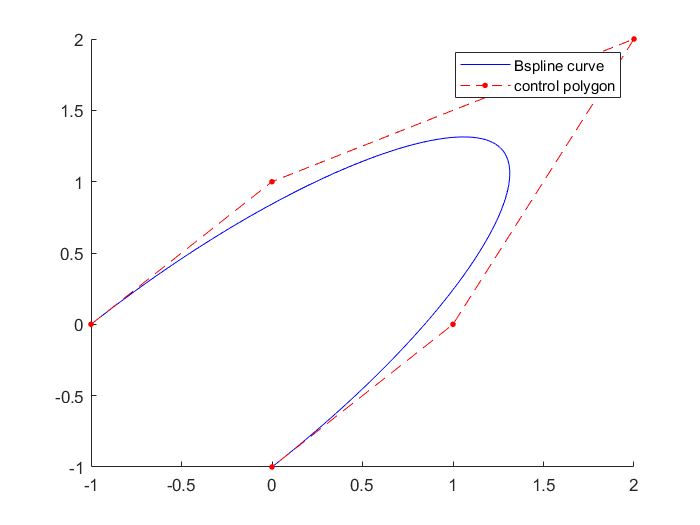
\includegraphics[width=0.8\textwidth]{bspline_2d_1.png}
        \label{fig: bspline_2d_1}
        \caption{控制顶点
        $p_0=(-1,0)', p_1=(0,1)', p_2=(2,2)', p_3=(1,0)', p_4=(0,-1)'$}
    \end{figure}
    \begin{figure}[H]
        \centering
        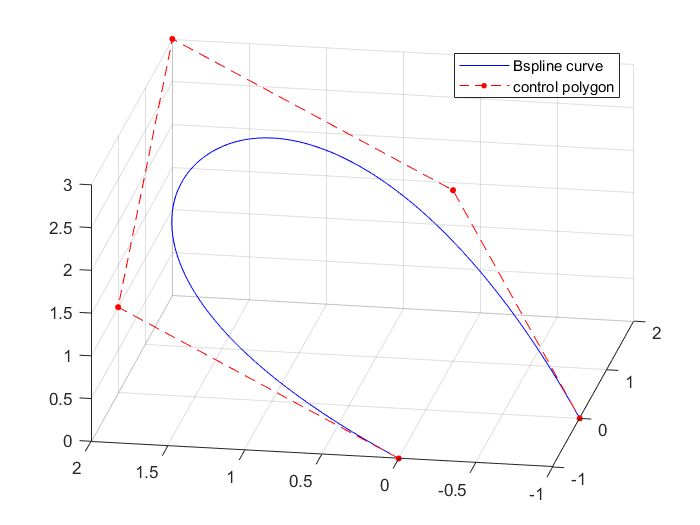
\includegraphics[width=0.8\textwidth]{bspline_3d_1.png}
        \label{fig: bspline_3d_1}
        \caption{控制顶点
        $p_0=(-1,0,0)', p_1=(0,2,1)', p_2=(2,2,3)', p_3=(1,0,2)', p_4=(0,-1,0)'$}
    \end{figure}
    \item 次数$p=2$,节点向量$u = [0, 0, 0, 1/3, 2/3, 1, 1, 1]$
    \begin{figure}[H]
        \centering
        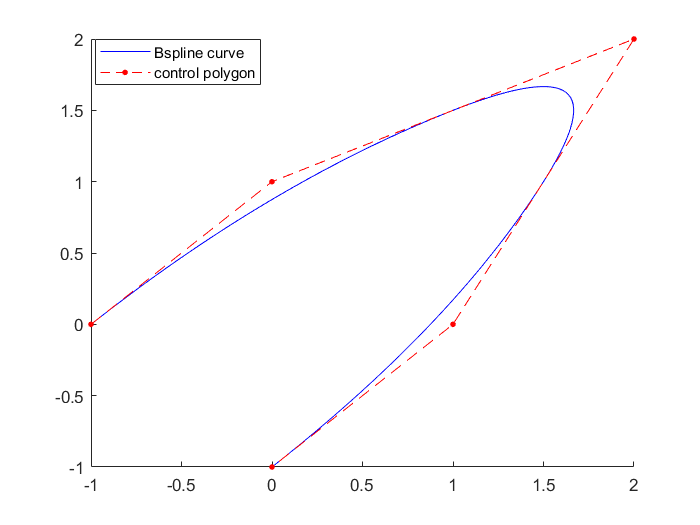
\includegraphics[width=0.8\textwidth]{bspline_2d_2.png}
        \label{fig: bspline_2d_2}
        \caption{控制顶点
        $p_0=(-1,0)', p_1=(0,1)', p_2=(2,2)', p_3=(1,0)', p_4=(0,-1)'$}
    \end{figure}
    \begin{figure}[H]
        \centering
        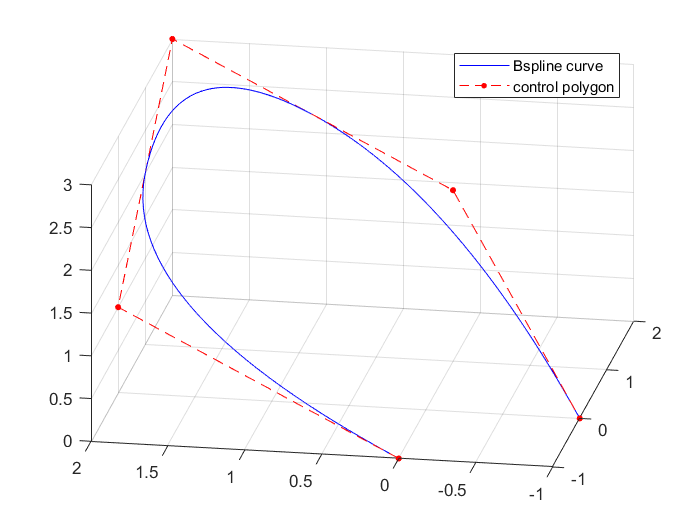
\includegraphics[width=0.8\textwidth]{bspline_3d_2.png}
        \label{fig: bspline_3d_2}
        \caption{控制顶点
        $p_0=(-1,0,0)', p_1=(0,2,1)', p_2=(2,2,3)', p_3=(1,0,2)', p_4=(0,-1,0)'$}
    \end{figure}
\end{itemize}

\subsection*{2.}
采用不同的参数化方法实现三次B-spline曲线插值,分别为均匀参数化、累积弦长参数化和切比雪夫累积弦长参数化\footnote{参考《数据插值中的参数化新方法》},并比较插值效果。\par
型值点:$p_0=(-1,0)', p_1=(0,1)', p_2=(2,2)', p_3=(1,0)', p_4=(0,-1)'$,
边界导矢:$D1 = (7.0990, 7.0990)', D2=(-7.0990, -7.0990)'$。
\begin{figure}[H]
    \centering
    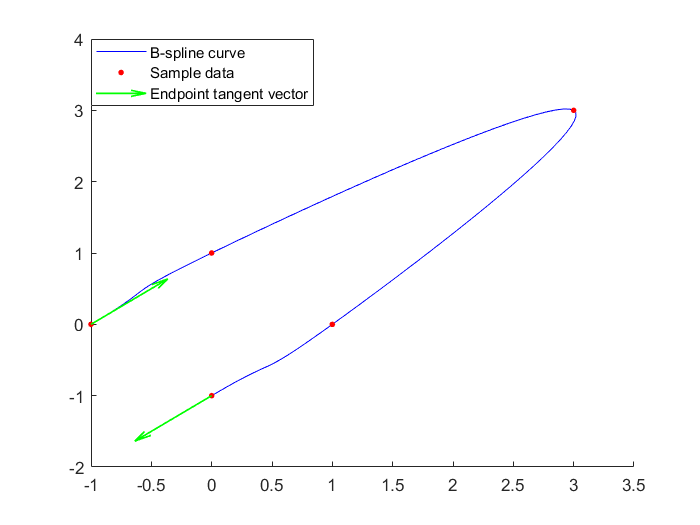
\includegraphics[width=0.8\textwidth]{cubic_bspline_interp_uniform.png}
    \label{fig: cubic_bspline_interp_uniform}
    \caption{均匀参数化}
\end{figure}
\begin{figure}[H]
    \centering
    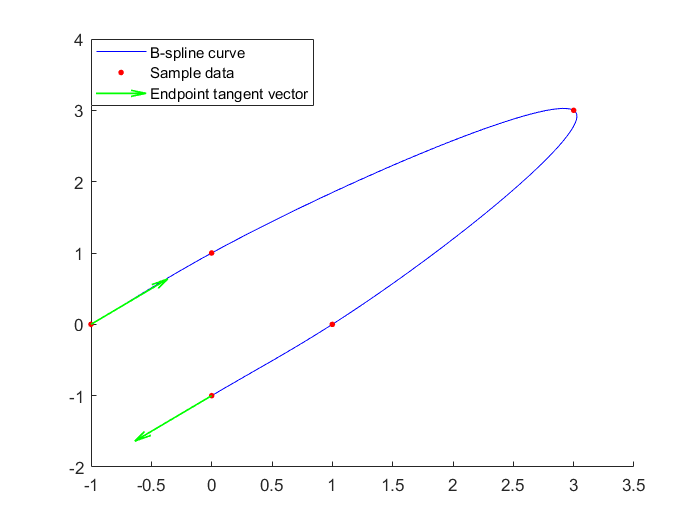
\includegraphics[width=0.8\textwidth]{cubic_bspline_interp_chord.png}
    \label{fig: cubic_bspline_interp_chord}
    \caption{累积弦长参数化}
\end{figure}
\begin{figure}[H]
    \centering
    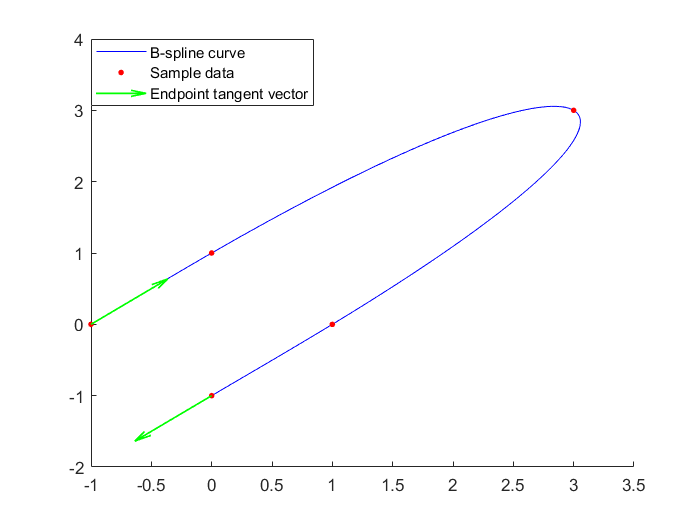
\includegraphics[width=0.8\textwidth]{cubic_bspline_interp_cheby.png}
    \label{fig: cubic_bspline_interp_cheby}
    \caption{切比雪夫累积弦长参数化}
\end{figure}


\end{document}
